%% LyX 2.2.1 created this file.  For more info, see http://www.lyx.org/.
%% Do not edit unless you really know what you are doing.
\documentclass[british,english]{article}
\usepackage[T1]{fontenc}
\usepackage[latin9]{inputenc}
\usepackage{geometry}
\geometry{verbose,tmargin=2cm,bmargin=2cm}
\usepackage{babel}
\usepackage{graphicx}
\usepackage{subcaption}
\usepackage{amsmath}
\usepackage{amsthm}
\usepackage[unicode=true]
 {hyperref}

\makeatletter
%%%%%%%%%%%%%%%%%%%%%%%%%%%%%% Textclass specific LaTeX commands.
\numberwithin{equation}{section}
\numberwithin{figure}{section}

%%%%%%%%%%%%%%%%%%%%%%%%%%%%%% User specified LaTeX commands.
\usepackage{braket}

\@ifundefined{showcaptionsetup}{}{%
 \PassOptionsToPackage{caption=false}{subfig}}
\usepackage{subfig}
\makeatother

\begin{document}

\title{Manual of RyMoP }

\author{Ke Liao\thanks{Any questions or queries should be addressed to \protect\href{mailto:ke.liao.whu@gmail.com}{ke.liao.whu@gmail.com}}}

\maketitle
\tableofcontents{}

\newpage

\section{Introduction}

RyMoP refers to Rydberg Molecule Potential \foreignlanguage{british}{Program}me
which is written in C++ and developed by Ke Liao for the 5. Physikalisches
Institut, Universit\"at Stuttgart. The programme can calculate the
potential in a Rydberg Molecule using the partial wave scattering
theory, to be precise only S- and P-wave scattering are included.
The programme, though at a primitive stage (no graphic interface or
post-process scripts), includes all the core functions needed to calculate
the S- and P-wave scattering Rydberg Molecule potential. Currently,
the programme has only been tested on Linux (Ubuntu) and Mac OSX with
gcc (g++) compiler 4.8 and it works flawlessly. Older version of gcc
like 4.2 may not support some features and newer versions like gcc
5 abandons some old features so that the programme cannot be compiled.
So choose gcc 4.8 to make life easier.

The programme comes with a compressed file, \emph{RyMoPP.tar.gz},
which when uncompressed will give you 4 folders: \emph{Code, Wave,
Scripts }and \emph{EigenLib}. All of the essential codes are stored
in \emph{Code}, \emph{EigenLib }is the \href{http://eigen.tuxfamily.org/index.php?title=Main_Page}{Eigen Library},
\emph{Scripts }contains some pre- and post-processing scripts and
\emph{Wave }contains a selected range of wave functions that you can
use. If you want to use more wave functions, you have to copy the
corresponding files into this folder. One important thing to note
is that the names of the newly copied files have to have the same
format as the old ones which are already there. Originally I obtain
those wave function files by converting the {*}.mat files to {*}.txt
files. I wrote a script called \emph{convert.py} to do this job. I
will address more about this script later in Scripts \ref{subsec:Scripts}. 

For record, I list the essential files here and explain briefly what
they do. 

\paragraph{Core Files}
\begin{enumerate}
\item \emph{Kore.cpp}, which is the core file in this programme and contains
all the essential functions;
\item \emph{specfunc.h}, which contains a collection of special functions,
including the Spherical Harmonics and another Spherical Harmonics
without $\sin\theta$\footnote{I will introduce this function in detail. It is crucial to the P-wave
scattering calculation.}. Though it is not included directly in Kore.cpp, it is contained
in 'integral.h';
\item \emph{memalloc.h}, which handles memory allocation. It is used in
'integral.h';
\item \emph{integral.h}, which provides integration of 3D angular integration.
In this file, it includes 'memalloc.h' and 'specfunc.h'. 
\item \emph{line.h}, which provides the functions used in 'Kore.cpp' to
read data files correctly.
\item \emph{compile.sh}, which is used to compile the programme. In this
file, it compiles the Kore.cpp with the option linked to the 'EigenLib'
library, which handles the matrices manipulations.
\end{enumerate}
%

\paragraph{Scripts\label{subsec:Scripts}}

Above 5 files are the essential ones. During the process, I also wrote
two python scripts, which are 
\begin{enumerate}
\item convert.py, which can convert the wave function files from {*}.mat
format to {*}.txt format, and the latter is the format that this programme
can read. Users have to pay attention to the format of the files'
name and the files themselves. The converted wave function files have
the eigenenergy of this state at the end of the file.
\item get\_pot.py, which is the post-processing script to get data from
the output files from the main programme.
\end{enumerate}
%
The implementation of the code involves some theoretical derivations,
so the next section is dedicated to the basics of the theory. After
that, I will dive into the details of the codes. In the end, some
exmples will be shown.

\section{Theoretical Basis}

In this section, we go through the basics of the theory. The system
under consideration is a Rydberg molecule, which consists of a Rydberg
atom and a ground state atom sitting in the range of the former. Due
to the scattering between the Rydberg electron and the ground state
atom, an effective attraction between these two atoms can form. Our
goal is to calculate the effective potential between the Rydberg atom
and the ground state atom when the distances between them changes.
The distance here refers to the distance between the ground state
atom and the nucleus of the Rydberg atom. The general idea is to expand
the scattered electronic wave function with the unperturbed eigenfunctions
from the isolated Rydberg atom, based on the linear variational principle,
we can get the perturbed electronic wave function and energy, in turn,
the energy of the electron acts as an effective potential for the
ground state atom in a wave similar to the Born-Oppenheimer approximation
in solids. 

\subsection{Atomic Wave Functions}

Firt of all, we need the unperturbed wave functions of a isolated
atom to be the basis functions. Consider the Schr\"odinger equation
for a Rydberg atom: 

\begin{equation}
\left[\frac{{\bf p}^{2}}{2m_{e}}+V_{mod}(r)\right]\Ket{\Psi}=E\Ket{\Psi},
\end{equation}
where $V_{mod}(r)$ is a efffective potential and we split the wave
function into radial and angular part
\begin{equation}
\Psi(r,\theta,\phi)=R({\bf r})\tilde{Y}(\theta,\phi).
\end{equation}
In the internal wiki of Pi5, there is a detailed explanation about
how to get the raidal part of the wave function, so we will skip this
part here. But we have to point out that the final calculated result
in the wave function file is only the radial part and it is not directly
stored as $r$ and $R(r)$, instead a transform of the variables is
used:

\begin{equation}
\begin{aligned}
x&=\sqrt{r},\\
X(x)&=x^{3/2}R(r).
\label{equ:trans}
\end{aligned}
\end{equation}As for the angular part, since we take the spin orbital interaction
into account, spinors, which are the conbinations of two spherical
harmonics, should be used here.

\begin{equation}
\begin{aligned}
\tilde{Y}_{(j-\frac{1}{2},\frac{1}{2})jm}&=\left(\sqrt{\frac{j+m}{2j}}Y_{j-\frac{1}{2},m-\frac 12}, \sqrt{\frac{j-m}{2j}}Y_{j-\frac 12,m+\frac 12}\right),\\
\tilde{Y}_{(j+\frac{1}{2},\frac{1}{2})jm}&=\left(-\sqrt{\frac{j-m+1}{2j+2}}Y_{j+\frac{1}{2},m-\frac 12}, \sqrt{\frac{j+m+1}{2j+2}}Y_{j+\frac 12,m+\frac 12}\right).
\label{equ:spinors}
\end{aligned}
\end{equation}

\subsection{Pseudopotential in Molecular Hamiltonian}

For a highly excited Rydberg atom interacting with a ground state
atom, the Hamiltonian is

\begin{equation}
H=\frac{{\bf P}^{2}}{M}+H_{el}+V_{n,e}({\bf r,R})
\end{equation}
where $H_{el}$ is the atomic Hamiltonian we mentioned in last subsection,
$M$ is the mass of the atom, ${\bf P}$ and ${\bf R}$ are the relative
momentum and position of the ground state atom with respect to the
ionic core of the Rydberg atom respectively and ${\bf r}$ is the
relative position of the Rydberg electron to the ionic core. $V_{n,e}({\bf r,R})$
is the famous Fermi-Pseudopotential:

\begin{equation}
V_{n,e}({\bf r,R})=2\pi A_{s}[k(R)]\delta({\bf r}-{\bf R})+6\pi A_{p}^{3}[k(R)\overleftarrow{]\nabla}\delta({\bf r}-{\bf R})\overrightarrow{\nabla}
\end{equation}
where $A_{s}(k)=-\tan[\delta_{0}(k)]/k$ and $A_{p}^{3}(k)=-\tan[\delta_{1}(k)]/k^{3}$
denote the energy-dependent griplet s- and p-wave scattering lengths.
It is worth pointing out that $\delta_{l=0,1}(k)$ are the energy
dependent phase shifts and $\frac{k(R)^{2}}{2}=E_{kin}=-\frac{1}{2}n^{*2}+\frac{1}{R}$
where $n^{*}$ is the effective principal quantum number. Unfortunately,
we do not have analytical expressions for $\delta_{l=0,1}(k)$ , so
we have to do a fitting based on the data we have got. See figure
( ) for an example of $N=35$. 


\begin{figure}
\centering
\begin{subfigure}[h]{0.45\linewidth}
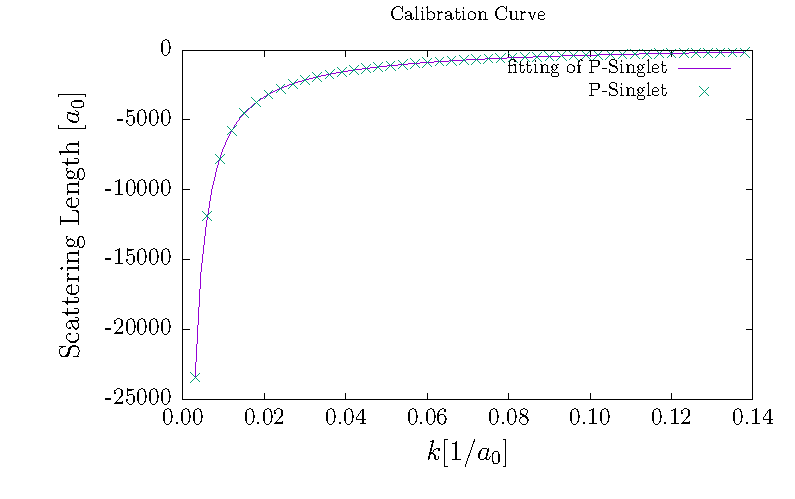
\includegraphics[width=\textwidth]{./Figs/PSinglet}
\end{subfigure}
\begin{subfigure}[h]{0.45\linewidth}
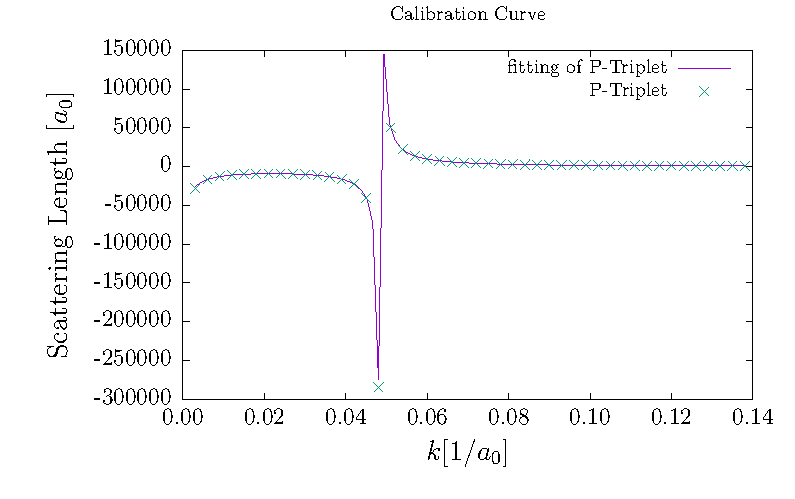
\includegraphics[width=\textwidth]{./Figs/PTriplet}
\end{subfigure}
\end{figure}

\end{document}
